\documentclass[11pt]{article}
\setlength{\parskip}{1em}
\setlength{\parindent}{0cm}
\usepackage[hmargin=2.2cm,vmargin=2.3cm]{geometry}
\usepackage{url}
\usepackage{hyperref}
\usepackage{breakurl}
\usepackage{float}

% For footnotes
\usepackage{endnotes}
\let\footnote=\endnote

\ifx\pdftexversion\undefined
\usepackage[dvips]{graphicx}
\else
\usepackage[pdftex]{graphicx}
\DeclareGraphicsRule{*}{mps}{*}{}
\fi

\begin{document}

\title{WebApps Group Project - Integrated Event Management and Discovery System for members of Imperial College London}

\author{Harry Lachenmayer, Artur Spychaj, Alex Rozanski and Thomas Rooney}

\date{\today}         % inserts today's date

\maketitle            % generates the title from the data above

\section {Introduction}

Our web app is a tool to help Imperial students find out about events happening on campus.

Most people currently find out about events on campus through noticeboards and mailing lists. The problem with these is that there is no easy, centralised way of finding out what is happening on campus. A big problem with the noticeboards is that a lot of the posters are outdated, and often irrelevant. It is also difficult to find out which mailing lists to subscribe to to find interesting events. Additionally, the Imperial College home page and the Union website have event calendars. An 'Imperial Mobile' application exists, which pulls data from the Imperial and Union sites, but we found that very few people use this, as it is complicated and slow.

\subsection{Requirements}

Our main aim is to bring all these disparate sources together and make a simple, 'one-stop' solution to find interesting events.

To achieve this, we identified three main requirements for the design of the app. The app should be:

\begin{itemize}
\item Simple \\ Users should immediately see relevant and interesting events. There should be no barrier of entry, such as registering or logging in, for most activities in the app.

\item Relevant \\ There are many different kinds of events happening on campus. Many of these are interesting to only a small subset of the college population. Users should be able to focus on events that are relevant to their interests.

\item Up to date \\ Advertising events on campus should be as easy as entering the event details once. Users should be able to stay up to date on the latest events without any effort.

\end{itemize}

We wanted to make the user interaction with the system as smooth as possible. To that end, we identified the following priorities:

\begin{itemize}
\item Authenticate with the college systems - no need to register a separate account. We consider this incredibly important because to attract a userbase from nothing we need to minimise the amount of interaction the user would need to do with the app to recieve useful information.

\item Provide automatic access to \textit{at least} the feeds that are already provided, such as the Imperial College Union \`Whats On\' calendar. We wanted to provide value without user interaction, so that it can be used immediately as an information source.

\item Provide user interactivity to provide information into the system. While the website as-is is intended to be a strong information source, the hope is that it provides an easier way to advertise events to members of the college, and that it could be a preferred platform for contacting people and cause a snowball effect in userbase increase. This requires that there are mechanisms available to add events.
\end{itemize}

\subsection {Target Audience}

The first stage of our project was defining our target user(s). We decided on limiting our users to members of the College, but we split these into the following sub-groups, and for each we created user stories describing their key characteristics:

\subsubsection{Undergraduate}
Harry is an undergraduate at Imperial College. He is a member of a few societies, but does not hold any executive committee positions. He likes going to events organised by the societies he is a member of, and other Union-organised events. He loves free stuff, especially free food, but usually finds out about events that give away free stuff far too late. He has a lot of friends that are really involved in societies, and is often invited to events by them through Facebook and society email lists. He is looking for an internship this summer. He was in halls in first year and knows a lot of people from there that he rarely sees anymore.

\subsubsection{Postgraduate}
Adam is currently doing his PhD in bio-chemistry. He attends many evening lectures relating to research topics that he is interested in. He is also a fan of classical music and likes to attend lunchtime concerts.

\subsubsection{Members of College Faculty}
\subsubsection{Event Organisers}
Lizzy is really involved in Union activities. She writes for Felix, and is the president of a mid-sized society. She is also the social secretary of another large society. She uses Facebook to invite people to nights out organised by these societies, and regularly uses the society email lists to announce society meetings and smaller events. She currently uses Google Docs spreadsheets to manage attendance to these smaller events.
a
\section {Project Management}

\subsection {Group Structure}

We split our group into two teams: one consisting of Alex and Harry, who worked on the client side, and the other consisting of Tom and Artur, who worked on the server-side implementation. Artur additionally implemented a scraper at the beginning of the project which collected event information from the Union calendar.

\subsection{Implementation Technology Decisions}

In implementing this we wanted to experiment somewhat with many of the new technologies that are only recently entering mainstream use. We focus here on the reason why we picked the major technologies such as front and {back end servers, language choice and why we chose to use a graph based database.

\subsubsection{CoffeeScript}
We chose to develop our application using CoffeeScript, a programming language with a clean and elegant syntax which compiles down to JavaScript. We realised that building a rich web application would involve writing a lot of client-side JavaScript code. JavaScript however has many quirks, many of which are nicely dealt with in CoffeeScript. As one of the team members already had considerable experience using CoffeeScript prior to the project, it was an obvious choice for the client-side application code.

\subsubsection{Backbone.js}
On the client-side, we are using a popular JavaScript MVC library called Backbone. This library provides us with "hassle-free" model synchronisation with the server and useful ways of dealing with UI changes in our view code. It is a small library, and leaves a lot of freedom for implementation details. For example, it doesn't prescribe any particular templating engine. (We are using a templating language called Jade)

\subsubsection {Node.js}
We chose Node.js as server-side platform. Node.js is currently massively growing in popularity, and there are many useful libraries and frameworks which allow us to focus on writing application-specific code rather than the "plumbing". Using Node.js also enabled us to develop both the front-end and back-end in CoffeeScript.

The Node.js server exists mainly to expose a REST interface to the client. We are using a library called Swagger, which lets us define our REST interface in the form of an "executable specification", greatly simplifying our server-side code.

\subsubsection {Nginx}
Nginx (pronounced engine-x) is a reverse-proxy web server first, and HTTP web server second. However, we decided to use it for our front-end web server because of its simple configuration, particularly that related to proxying. 

All the front-end API calls are made to the nginx server which then proxies them to the back-end Node.js server. This has the advantage of creating a clean separation between the front- and back-ends of our project, and by proxying the API calls doesn't expose the back-end API server publicly. 
\subsubsection {Neo4j}

Neo4j is one of the leading graph based databases. It's an open-source, high-performance, NOSQL database that's been seen more and more in both startups and enterprise software systems. We chose it because the data we wish to store and mine for information is essentially a graph. For example each event is connected to users associated with them, multiple tags, API keys for authentication as well as potentially more, with many optional fields (see image). We felt that this sort of dataset fits the graph-based database paradigm much better than a relational database, and were excited to get to use some new technologies.

In practice, this has worked out well for us, because it ensures that our querying of the database is much faster than could be achieved on a relational database of similar specifications, because we can start off each query and only be at most 5 edges away from the nodes and thus the information we want. It also fits JSON data well, as each node operates as a key-value store, and is instantly convertable using the client libraries to its REST API.

TODO: Add image of database graph.
\subsection {Design Processes}

Throughout the project, we took both an agile approach by continuously iterating on ideas, but also planned heavily up-front before we started development to establish our target users and the design of our project. This was very important to us as the cost and ease of making changes to a project are lower the earlier they are made.

We started out by creating a business model canvas, which allowed us to think about aspects to the project such as the target audience and the viability of our project as a product. We also devised user stories for our target users to get a better understanding of the problems they face and how our project would address these.

Still before we'd even written a single line of code, we designed the user interaction and a rough outline for the user interface. We iterated on designs and mockups until we had a workflow and experience that we were happy with.

At this point, we decided on which technologies to use to build our project with for both the front-end and back-ends. We then started to implement features and iterated on them until we were happy with the result. Although we split ourselves into two teams (for the front-end and back-end), we made sure to constantly integrate both parts to find and fix issues as early as possible during the development process.

\subsubsection {Ethical impact}
	Security, passwords etc
aa
\subsection {Collaborative Tools}
\subsubsection {GitHub Wiki}
We used the GitHub Wiki as a place to document areas of the project as we implemented them. For example, both the client-side and server-side teams each documented the process involved in setting up their respective system, so that other group could always run the entire system to test the part they were working on with the other components.

We also created Wiki entries for the REST API specification as it was being implemented server-side. This meant that the client-side group could interact with it and start testing calls to it as early as possible.
\subsubsection {Trello}

Trello\footnote{\url{http://trello.com}} is an organisational and management web application produced by FogCreek. It provides a collection a lists of items, each of which can be thought of as a list of small items (which can be expanded in more detail underneath).

\begin{figure}[H]
\centering
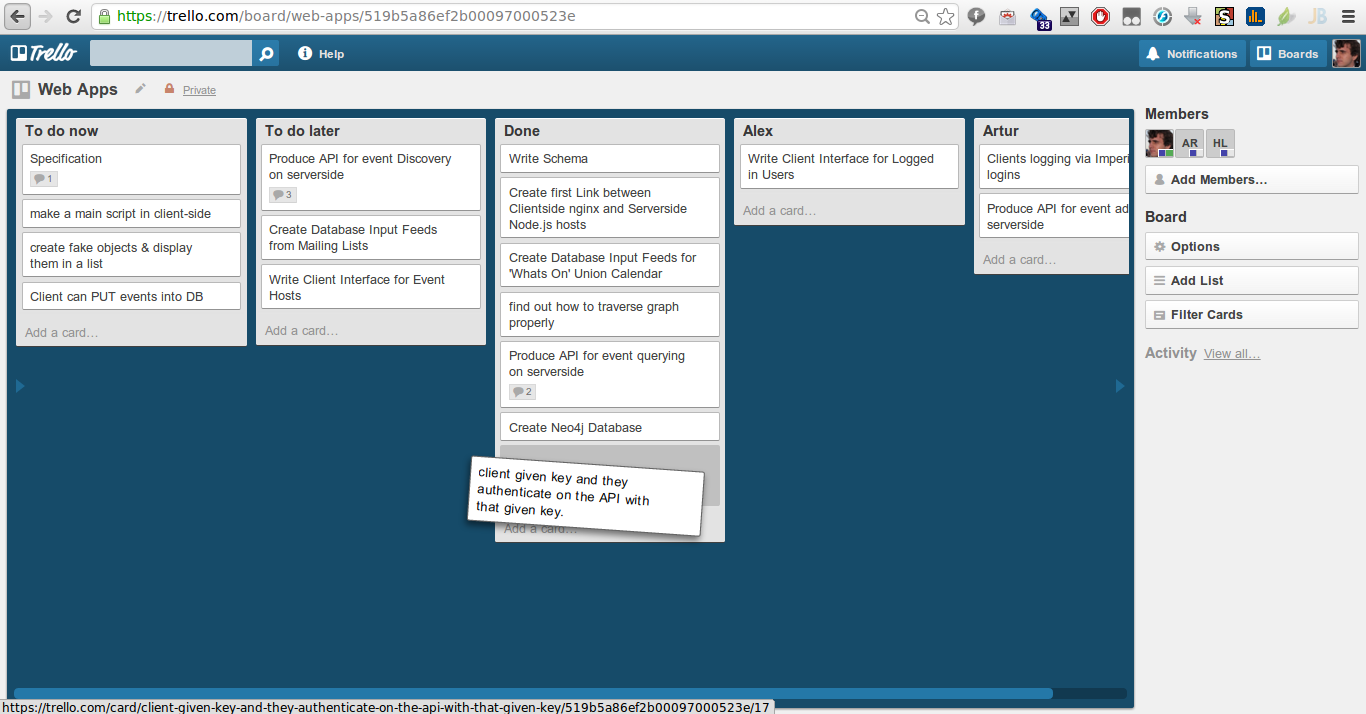
\includegraphics[scale=0.35]{trello.png}
\caption{\label{fig:trello} Trello - Collaborative Organizational Tool}
\end{figure}
In following the Agile development methodology of an iterative development, we used Trello to define new tasks during our group meetings. In doing this, we could effectively ensure that there was fair and consistent contribution from all members by assigning each task to somebody on Trello. This also allowed us all to keep track of where we were in the project, an maintain a consistent list of tasks we needed to do, minimizing the `what now?' time.


\subsection {Version Control System}
a
\section {System Description}

[Introduction]

\subsection {Core Features}

When a user first uses the device, what they see is all events that are occuring on that day, scrolling forward through time. Each event item acts as a button through which they can find out more about that event.

\subsection {Social Features}
\subsubsection {Tags}
\subsubsection {Follower System}
\subsubsection {Friends}
\subsubsection {Groups}
\subsection {Other Features}
\subsubsection {Subscription}
\subsubsection {Notifications}

Email Blah

\section {System Implementation}
\subsection {Front End}
\subsection {Back End}

The backend is implemented with a Node.js server, allowing simple communciation and reusable code between backend and frontend. We split the project down into several categories, which we kept seperate from each other to minimize rigidity.

\subsubsection {API}
	For the main API, we run express\footnote{express.js}, a common package that has many plugins for enhanced ease of use in building web applications. On top of this we are running Swagger, a package built to ease documentation and design of RESTful interfaces. Swagger's major advantage is a one-command documentation/validator of the API, by running its validator and static documentation tool\footnote{https://github.com/wordnik/swagger-codegen} on the Node.js code itself. This allows us to perform basic unit testing to validate the UI whilst describing the UI for its documentation.
	Swagger also provides an authentication callback, however we decided not to use this. We did this because the major limitation of its `validator' authentication callback is that it gets added to every HTTP request to authenticate it individually. We didn't want to do this, and instead split between HTTPS requests for logged in sessions, with user personalisation and extra permissions, and the public HTTP web application, which simply provides a simple way to view the upcoming calendar of public events. For authentication we used the Kerberos system, which ensured only college users could access the system.

\subsubsection {Crawler}

There are already a few events that the Imperial already displays on their calendars.
However these are usually scattered accross the Imperial website.
Given that the union calendar does not provide any API to access the database with the list of events then it is necessary to fetch these events directly from the website.
In order to extract the relevant information the \textit{cheerio} framework was use.
It is a framework that allows to operate on the HTML dome in a similar fashion to the jQuery framework.

On a more positive side the events for the Imperial Website are returned using the RSS format.
Using the node.js package \textit{feedparser} the fetched data was parsed into a JSON format.
The JSON format was later converted into the relevant calendar format used by the Neo4j database.

\subsubsection {Notifications}
	Email notifications are one of the services we provide for registered users. Each week, or other configured time, we collate the users subscriptions and send the upcoming events to them in an email. This is implemented via a connection to an SMTP server, a mining of the users subscribed events via a Cypher query, followed by a prettifying on the events and parsing into a HTML email via a templating engine.
\subsubsection {ICAL}

In order to allow the users to view the events even outside of our website the events list can easily be exported into the iCal format. This is the standard format used to display calendar events and is currently supported by online websited such as outlook and gmail as well as multiple desktop applications.

Given that each of these formats requires a publicly availiable URL the events server generate a random string for each user. This URL can then be used to receive a calendar of all events to which he subscribed. However the user can easily opt out from the URL as well as create a new one.

This method allows a user to quickly synchronize with the events from the Imperial website and see them in native applications that he uses.

\subsubsection {Database stuff}

The Neo4j database is a graph database that allows to quickly traverse the database.
Our database consists of a root node which has edges to nodes that are treated as `database tables'.
Creating a node for each table increases the search time. An alternative would be to create and index for each table node. This has the advantage of not having to specify a node that is treated as a root node.
The tables contain entries to relevant nodes (users, events, groups, etc.) that contain the relevant information saved as JSON data. Being stored in JSON format it is compatible with Node and the database can easily be upgraded. It is not necessary that all of the nodes in a given `table' have the same keys.

Nodes are connected by edges to define relationships like \textit{Friendship}, \textit{Following}, \textit{Member_Of}.

\subsubsection {Problems or Limitations}
	
	Time, Cypher Queries, SSL Password stuff (self-signed not good)



\section {External Packages}
On the client-side, we used Component\footnote{http://github.com/component/component}, which is a client-side package manager. It bundles reusable JavaScript, CSS and HTML into 'components', modules which can be reused in multiple places. 

We used serveral external client-side components:
\begin{itemize}
    \item \textbf{Backbone}\footnote{http://github.com/solutionio/backbone}: a minimal MVC library.
    \item \textbf{ListJS}\footnote{http://github.com/cayasso/list}: a JavaScript library which makes HTML lists sortable, filterable and searchable.
    \item \textbf{jQuery}\footnote{http://github.com/component/jquery}: a JavaScript library which adds many utilities including finding DOM elements by CSS-like selectors.
    \item \textbf{jade-runtime}\footnote{http://github.com/monstercat/jade-runtime}: the component used to evaluate Jade\footnote{Jade Template Engine: http://jade-lang.com} templates.
    \item \textbf{Underscore}\footnote{http://github.com/component/underscore}: a utility library used extensively with Backbone.
    \item \textbf{Moment}\footnote{http://github.com/component/moment}: a JavaScript date library making tasks such as formatting easier.
    \item \textbf{Reset}:\footnote{http://github.com/ianstormtaylor/reset}: a CSS reset component. 
\end{itemize}

\subsection{Common}
\begin{itemize}
\item Node
\item Coffeescript
\end{itemize}

\subsection{Backend}
\begin{itemize}
\item Neo4j
	\subitem everything in package.json
	\subitem more everything
\end{itemize}
\subsection{FrontEnd}
\begin{itemize}
	\item Nginx
\end{itemize}

\section {Conclusion}




\newpage

\theendnotes

\end{document}

